%%%%%%%%%%%%%%%%%%%%%%%%%%%%%%%%%%%%%%%%%%%%%%%%%%%%%%%%%%%%%%%%%%
%% MDPI Insects manuscript -- ACS (numbered) citation style
%%%%%%%%%%%%%%%%%%%%%%%%%%%%%%%%%%%%%%%%%%%%%%%%%%%%%%%%%%%%%%%%%%
\documentclass[insects,article,submit,pdftex,moreauthors]{Definitions/mdpi}

%% Extra packages (beyond what mdpi.cls loads)
%% Note: mdpi.cls already loads hyperref, natbib, booktabs, tabularx, etc.
\usepackage{longtable}
\setlength{\headheight}{20pt}

%% ------------------------------------------------------------------
%% Journal / article metadata
%% ------------------------------------------------------------------
\firstpage{1}
\makeatletter
\setcounter{page}{\@firstpage}
\makeatother
\pubvolume{1}
\issuenum{1}
\articlenumber{0}
\pubyear{2026}
\copyrightyear{2026}
\datereceived{}
\daterevised{}
\dateaccepted{}
\datepublished{}

\corres{Correspondence: knessen@calpoly.edu (K.N.)}

%% ------------------------------------------------------------------
%% Title
%% ------------------------------------------------------------------
\Title{Wind Does Not Disrupt Overwintering Monarch Butterfly Clusters: Direct Empirical Test of a Three-Decade Management Assumption}

%% ------------------------------------------------------------------
%% Authors
%% ------------------------------------------------------------------
\Author{Kyle Nessen \textsuperscript{1,*}, Peter C. Ibsen \textsuperscript{2}, Jay E. Diffendorfer \textsuperscript{2} and Francis X. Villablanca \textsuperscript{1}}

\AuthorNames{Kyle Nessen, Peter C. Ibsen, Jay E. Diffendorfer and Francis X. Villablanca}

\address{%
\quad \textsuperscript{1} Biological Sciences Department, California Polytechnic State University, San Luis Obispo, CA 93407, USA;
\quad \textsuperscript{2} U.S. Geological Survey, Geosciences and Environmental Change Science Center,  Denver, CO 80225, USA}

%% ------------------------------------------------------------------
%% Simple Summary (required by Insects)
%% ------------------------------------------------------------------
\simplesumm{The population size of monarch butterflies in the western U.S. has been declining since the 1980s. This population of butterflies spends the winter months in groves of trees along the California coast. Habitat management in these groves has focused on controlling wind, as wind was thought to negatively affect monarchs. Though this seemed like a good idea, this paper finally tested it. We find that wind itself does not have any negative effects and therefore does not need to be controlled. Instead, we find that sunlight and wind interact. This is likely because sun and wind interact to both warm and cool monarch butterflies. This new finding could change the way in which we manage groves. Instead of managing or suppressing wind, combinations of wind and light should be provided within the groves, so that monarch butterflies can choose among suitable thermal conditions for overwintering.}

%% ------------------------------------------------------------------
%% Abstract
%% ------------------------------------------------------------------
\abstract{The western monarch butterfly (\textit{Danaus plexippus}) population has declined by over 99\% since the 1980s, making conservation of overwintering habitat a management priority. For three decades, conservation has relied on a Microclimate Hypothesis, including a nested Wind Disruption Hypothesis that associates wind speeds above 2~m/s with roost abandonment. We deployed cameras and wind sensors at two overwintering groves during the 2023--2024 season to track visible cluster size and nearby wind conditions across 80 days. We did not detect a consistently negative association between maximum wind gust and subsequent change in visible Butterfly Index. In the 30-minute analysis, the association depended jointly on approximate local temperature and sun-exposed BI. Gusts were associated with declining BI under cool, sunny conditions and increasing BI under warm, sunny conditions, while conditional wind slopes were not distinguishable from zero when sun-exposed BI was zero. A Next Day Window analysis also supported a conditional wind by sun-exposed BI relationship, with greater model-selection uncertainty. These observations do not provide an exact test of sustained exposure above 2~m/s, but they do not support a simple, universal wind-disruption response under the monitored conditions. The conditional patterns motivate direct tests of thermoregulation as a possible mechanism.}

%% ------------------------------------------------------------------
%% Keywords
%% ------------------------------------------------------------------
\keyword{clustering behavior; conservation; \textit{Danaus plexippus}; habitat management; microclimate; overwintering; thermoregulation; western monarch butterfly; wind disruption}

\externalbibliography{yes}

%% ===================================================================
\begin{document}

%% ------------------------------------------------------------------
\section{Introduction}
%% ------------------------------------------------------------------

The distribution and survival of invertebrate species are governed by complex interplays of biotic and abiotic factors. While biotic interactions influence community assembly in part through predation, competition, and parasitism \cite{blois-heulinDirectIndirectEffects1990,laffertyComparingMechanismsHost2013,miller-terkuilePredatorPreyInteractions2022}, abiotic conditions often set the fundamental limits determining where invertebrates can persist \cite{sextonEvolutionEcologySpecies2009,louthanWhereWhenSpecies2015,thomasClimateChangeRange2010}. Temperature constrains invertebrate physiology across all latitudes, from Antarctic midges \cite{everattResponsesInvertebratesTemperature2015} to desert land snails \cite{schweizerSnailsSunStrategies2019}. In invertebrates, temperature correlates positively with metabolic rates and respiratory water loss, creating compound stresses that limit activity windows \cite{chownWaterLossInsects2011}. In addition, via a correlation with temperature, solar radiation can drive both direct physiological impacts and behavioral responses. Examples range from army ants demonstrating habitat-specific thermal maxima tied to insolation exposure \cite{baudierExtremeInsolationClimatic2018}, to terrestrial gastropods climbing vertical surfaces to escape ground-level heat \cite{schweizerSnailsSunStrategies2019}.

Wind is another abiotic factor that can influence invertebrate distribution and behavior through remarkable and diverse mechanisms that vary across species. For example, cockroaches perceive air currents as low as 0.015--0.03~m/s and demonstrate predictable orientation shifts in response to wind velocities \cite{bellSearchAnemotacticOrientation1979}. Mosquitoes' sensitivity to winds as light as 1.0~m/s can effectively ground entire populations \cite{bidlingmayerEffectWindVelocity1995}. Some species exploit wind for dispersal through specialized behaviors, such as spiders' stereotypical ``tiptoe'' behavior which initiates ballooning but only when winds permit controlled trajectories \cite{bonteHeritabilitySpiderBallooning2007}. Some species respond to wind as an environmental stressor requiring active avoidance. For mad hatterpillar larvae, 3~m/s winds are a disturbance cue, triggering movements to stable microsites on branches, and behavioral shifts to leeward sides and abaxial leaf surfaces \cite{leonardExposureWindAlters2016}. Underlying many of these behavioral avoidance responses are the fundamental thermal and hydric effects of wind, as convective cooling from air movement significantly alters both heat and water exchanges between organisms and their environment, particularly when wind interacts with solar radiation \cite{riddellWindNicheThermal2025}. For example, in butterflies, basking is used to warm at cool temperatures. But wing position can be modified to reflect solar energy towards the thorax, or to minimize convective heat loss and maximize solar radiation heat gain of the wing itself, causing antennae, wings and thorax to heat up at different rates and reach different temperature above ambient (reviewed by \cite{munroClimateStrongPredictor2019,tsaiPhysicalBehavioralAdaptations2020,krishnaAirTemperatureDrives2021}). Thus, wind can be recognized as having direct mechanical effects, and indirect thermal and hydric effects through interactions with covariates such as temperature and insolation.

The monarch butterfly (\textit{Danaus plexippus}) offers an exceptional system for studying how abiotic factors shape invertebrate ecology. Late summer environmental cues, such as shortening day length and cooling temperatures, trigger the emergence of a migratory monarch generation \cite{reppertDemystifyingMonarchButterfly2018,goehringEffectsPhotoperiodTemperature2002,hermanJuvenileHormoneRegulation2001,barkerEffectPhotoperiodTemperature1976}. These adults exhibit unique characteristics including reproductive diapause (suspended reproduction), and an elongated-wing long-travel-distance phenotype \cite{barkerEffectPhotoperiodTemperature1976,yangIntrapopulationVariationNatal2016,tuskesOverwinteringEcologyMonarch1978}. The fall migrants collect nectar en route thus building lipid reserves needed for overwintering \cite{hermanJuvenileHormoneRegulation2001,chaplinEnergyReservesMetabolic1982,Urquhart1978Autumnal}. And while Eastern monarchs travel to high-altitude oyamel fir (\textit{Abies religiosa}) forests in central Mexico, our focus, the Western monarch population, migrates to overwintering groves widely scattered along the Pacific coast of California \cite{browerUnderstandingMisunderstandingMigration1995,Urquhart1978Autumnal}.

While overwintering, roughly from mid-October through mid-March, monarchs survive on accumulated lipid reserves and associated thermoregulatory balancing \cite{chaplinEnergyReservesMetabolic1982,mastersMonarchButterflyDanaus1988}. As ectotherms, monarchs face a fundamental trade-off: maintain body temperatures cool enough through metabolic suppression to conserve energy for the entire overwintering season, yet warm enough to permit for bouts of essential flights \cite{mastersMonarchButterflyDanaus1988,chaplinEnergyReservesMetabolic1982,kammerThoracicTemperatureShivering1970,alonso-mejiaInfluenceTemperatureSurface1992}. Temperatures of 12.7--16.0$^{\circ}$C represent the minimum thoracic temperature required for powered flight \cite{mastersMonarchButterflyDanaus1988} and represent flight threshold temperature for (Eastern) monarchs. Below this threshold, monarchs employ behavioral thermoregulation either through dorsal basking, which can elevate body temperature to flight capability within 30 seconds of sun exposure, or through energetically costly shivering that consumes energy 25 times faster than resting \cite{mastersMonarchButterflyDanaus1988}. Thus ``warm enough'' can be environmentally or physiologically attained, but at significantly different costs to lipid stores. In terms of ``cool enough,'' direct sun exposure can rapidly elevate thoracic temperatures to 33.6$^{\circ}$C, forcing butterflies to adopt sun-minimizing postures or engage in heat-dissipating flights \cite{barkerEffectPhotoperiodTemperature1976}. This energetic balancing means that monarchs selecting overwintering sites must find locations that minimize both sustained freezing exposure (warm enough) and elevated metabolic expenditure (cool enough) \cite{mastersMonarchButterflyDanaus1988,alonso-mejiaInfluenceTemperatureSurface1992,calvertEffectRainSnow1983,andersonFreezeprotectionOverwinteringMonarch1996}.

Our focus on abiotic conditions, but more specifically wind, builds on early studies from Mexican overwintering sites that led Leong \cite{leongMicroenvironmentalFactorsAssociated1990} to propose the Microclimate Hypothesis for western monarchs overwintering in California. This hypothesis posits that monarchs select clustering locations within groves based on a measurable microenvironmental envelope characterized by four key parameters each with a specific benefit: wind protection or speeds below 2~m/s ($\sim$5~mph) preventing cluster disruption, cool temperatures maintaining diapause while minimizing freezing risk and elevated metabolic expenditure, dappled sunlight enabling behavioral thermoregulation, and high humidity or accessible moisture to prevent desiccation \cite{leongMicroenvironmentalFactorsAssociated1990,leongUseMultivariateAnalyses1991}. Wind emerged as particularly critical in Leong's Microclimate Hypothesis, and wind is the only parameter for which there is a proposed parameter value or range (below 2~m/s (5~mph), \cite{leongMicroenvironmentalFactorsAssociated1990,leongUseMultivariateAnalyses1991}).

Leong's initial studies measured wind speeds at trees with and without butterfly clusters, concluding that ``during winter storms, the butterflies clustered on those few trees that offered the greatest protection against winds of 2~m/s or greater'' \cite{leongMicroenvironmentalFactorsAssociated1990}. Though, technically the highest wind speed measured in this study was only 1.66~m/s. Based on these inferred correlations Leong reported that ``butterflies cluster in areas of the grove that offer exposure to filtered sunlight and shelter from strong wind movement'' \cite{leongUseMultivariateAnalyses1991}. In later publications, Leong added anecdotal observations, noting that ``roosting butterflies were blown from their clusters or dislodged by excessive branch movements (shaking) caused by winds exceeding 2~m/s'' and that ``upon dislodgment, the butterflies flew to and resettled on foliage of trees that offered better shelter from strong winds'' \cite{leongRestorationOverwinteringGrove1999}. When storm winds coincided with morning temperatures below 15$^{\circ}$C, ``the dislodged butterflies would be blown to the ground and remain there until temperatures reached flight threshold,'' with ``butterflies littering the ground at the base of roosting trees'' commonly observed after winter storms \cite{leongRestorationOverwinteringGrove1999}.

Though the Microclimate Hypothesis originated from untested anecdotal observations, it still gained widespread acceptance and came to directly inform management guidelines at multiple levels. Leong's 2016 synthesis for California Department of Fish and Wildlife formally established that ``winds $\geq$ 2~m/s are disruptive to the aggregating butterflies by blowing them from their roosting branches or dislodging them by shaking the branches,'' and that when subjected to such winds when above flight threshold temperature, butterflies ``either flew to a more sheltered area of the grove or, if no refuge area was available, abandoned the grove temporarily or for the remainder of the season'' \cite{leongEvaluationManagementCalifornia2016}. Thus, the Microclimate Hypothesis ``made obvious'' that successful overwintering sites would consistently exhibit a specific suite of conditions, including protection from wind $\geq$ 2~m/s. This then implied that specific abiotic parameters should guide habitat management and restoration efforts, a principle now widely adopted in monarch conservation plans \cite{xercessocietyStateMonarchOverwintering2016,jepsenProtectingCaliforniasButterfly2017,peltonMonarchButterflyOverwintering2020,weissRecommendationsRestorationMonarch2008,althouse&meadeinc.EllwoodMesaSperling2023}.

However, empirical testing has gradually dismantled the Microclimate Hypothesis' core assumption of a uniform environmental envelope. When researchers tested whether monarchs select for consistent microclimatic attributes (temperature, light, and humidity) across groves, they found that the realized microclimate varied significantly with latitude and local geography \cite{sanieeHierarchyScaleInfluence2022}. Temperature responses proved more complex than originally proposed, with monarchs avoiding freezing temperatures but selecting the warmest cold temperatures available at their latitude \cite{fisherMultiScaleSpeciesDistribution2024}. Humidity showed geographic variability rather than consistency \cite{sanieeHierarchyScaleInfluence2022}. This geographic variability in microclimate utilization, where selection seems to occur hierarchically across multiple spatial scales rather than for a single environmental envelope, fundamentally contradicts Leong's original hypothesis \cite{fisherMultiScaleSpeciesDistribution2024,sanieeHierarchyScaleInfluence2022}. Of the three Microclimate Hypothesis parameters tested thus far, only light exposure is supported as a potential unifying factor. Given that various research perspectives have been utilized in the consideration of light, successful overwintering sites are known by different light characteristics including consistent patterns of canopy openness \cite{weissForestCanopyStructure1991}, specific shading patterns \cite{ibsenDensityDependenceHabitat2026}, and high intensity light of short duration \cite{sanieeHierarchyScaleInfluence2022}.

Among the four parameters of Leong's Microclimate Hypothesis, the wind disruption component of the Microclimate Hypothesis (hereafter Wind Disruption Hypothesis) stands apart as never having undergone direct empirical testing. Therefore, despite widespread adoption of the Wind Disruption Hypothesis' 2~m/s wind protection threshold in restoration efforts \cite{xercessocietyManagingMonarchsWest2018,jepsenProtectingCaliforniasButterfly2017,althouse&meadeinc.EllwoodMesaSperling2023,u.s.fishandwildlifeserviceMonarchDanausPlexippus2024,weissAlbanyHillMonarch2018,leongEvaluationManagementCalifornia2016}, no study has directly tested butterfly responses to wind exposure, or distinguished whether butterflies actively avoid wind or the hydric or thermic effects of wind, or some other correlated but unmeasured variable(s).

Between the 1980s and mid-2010s, overwintering populations of western monarchs collapsed by approximately 97\% \cite{schultzCitizenScienceMonitoring2017}, with population viability analyses revealing a 72\% quasi-extinction risk within 20 years \cite{schultzCitizenScienceMonitoring2017}. The winter 2018 to 2019 Western Monarch Thanksgiving Count recorded fewer than 30,000 monarchs, a single-year drop of 86\%, representing over 99\% decline from 1980s abundance \cite{peltonWesternMonarchPopulation2019}. The 2020 count documented only 1,901 butterflies, the lowest number ever recorded. The 2024 to 2025 count of 9,119 represents the second-lowest count. The latest count in 2025--2026 of 12,260 is the third lowest on record and demonstrates the population's continued precarity \cite{xercessocietyWesternMonarchButterfly2025}. Declines are associated with multiple interacting stressors including herbicide use and associated breeding habitat loss, pesticide exposure, climate change, and the loss and degradation of overwintering habitat \cite{croneWhyAreMonarch2019,peltonWesternMonarchPopulation2019,oberhauser2026MonarchConservation}. In western monarchs evidence suggests that the overwintering stage represents the most limiting phase of the annual cycle, with declines concentrated during winter and early spring periods \cite{peltonWesternMonarchPopulation2019,mariniDensitydependenceDecliningPopulation2017}. Thus, in terms of Western Monarch conservation priorities, management of California coastal overwintering groves has emerged as the focal point, and testing the Wind Disruption Hypothesis has become critically important.

Testing the Wind Disruption Hypothesis requires addressing a fundamental methodological challenge: isolating wind effects from confounding environmental variables that naturally covary in field settings. Solar radiation is a potential covariate that can trigger butterfly departures through direct heating \cite{mastersMonarchButterflyDanaus1988,kammerThoracicTemperatureShivering1970}. Temperature is a potential covariate known to independently influence activity patterns, with monarchs exhibiting predictable responses as temperatures approach and exceed flight thresholds \cite{barkerEffectPhotoperiodTemperature1976}. Time of day creates inherent activity rhythms related to sun angle and thermal conditions \cite{mouritsenVirtualMigrationTethered2002} especially if clusters reform nightly. Furthermore, wind itself is multidimensional, characterized not only by average speed but also by gustiness and variability \cite{nathanLongdistanceBiologicalTransport2005} that could differentially affect butterfly behavior. A rigorous test must therefore control for potentially confounding factors while examining multiple aspects of wind exposure.
Our primary objective was to evaluate the Wind Disruption Hypothesis. We hypothesized that if wind disrupts overwintering aggregations, increasing wind exposure would predict declines in cluster size over immediate and next-day response windows. We evaluated this prediction while accounting for temperature, time of day, prior cluster size, and sun-exposed BI.


%% ------------------------------------------------------------------
\section{Materials and Methods}
%% ------------------------------------------------------------------

\subsection{Study Design and Sites}

We conducted an observational field study at Vandenberg Space Force Base (VSFB, 34.7398$^{\circ}$N, 120.5725$^{\circ}$W) in Santa Barbara County, California. VSFB contains 30 documented monarch overwintering groves, principally in mature blue gum eucalyptus (\textit{Eucalyptus globulus}) stands \cite{xercessocietyWesternMonarchThanksgiving2025}. Monitoring was attempted during the 2023--2024 and 2024--2025 overwintering seasons. The analyses use only observations from 17 November 2023 through 4 February 2024 because only two groves produced usable cluster time series. Monarch abundance during 2024--2025 was insufficient for a second season of analysis \cite{xercessocietyWesternMonarchThanksgiving2025}.

Spring Canyon (SC, Western Monarch Thanksgiving Count site 2712, 34.6315$^{\circ}$N, 120.6182$^{\circ}$W) is a 2.0-ha riparian grove of mature blue gum eucalyptus reaching approximately 40~m in height. A perennial creek, variable tree spacing, and heterogeneous understory create a structurally diverse grove. UDMH (Western Monarch Thanksgiving Count site 2822, 34.6719$^{\circ}$N, 120.5950$^{\circ}$W) is a 5.1-ha site composed of blue gum eucalyptus windrows with scattered low shrubs. Within the analytical season, equipment was repositioned as visible aggregations shifted, producing ten analyzed monitoring periods, hereafter deployments. Eight were at SC and two were at UDMH.

\subsection{Monitoring System and Deployment Units}

We mounted monitoring equipment on freestanding fiberglass telescopic poles with a maximum extension of 15~m (Max-Gain Systems, Inc., Marietta, GA) supported by triangular bases and guy lines. For analyzed deployments, the equipment was positioned 5.4--9.4~m above ground and 4.2--16.5~m horizontally from the monitored cluster. Pole height was selected to approximate the elevation of the visible roost area while maintaining an unobstructed camera view. Cluster height varied during observation periods and was not recorded systematically, so vertical sensor-to-cluster distances could not be calculated. Complete placement metadata are provided with the reproducibility materials.

GardePro E7 and E8 trail cameras (Shenzhen, China) were modified with near-infrared pass filters ($>$850~nm). Near-infrared imaging rendered clustered butterflies dark against bright eucalyptus foliage, increasing visual contrast \cite{gatesSpectralPropertiesPlants1965,hristovEstimatingOverwinteringMonarch2019,thajAnalysisOpticalProperties2025}. Cameras operated in time-lapse mode with motion detection disabled and remained fixed within each deployment. Images were acquired at deployment-specific intervals of 5 or 10 minutes and standardized to a 30-minute series by deterministic downsampling. Only daylight images were retained because passive near-infrared imaging required ambient light to distinguish butterflies reliably from foliage. Cameras were positioned with an unobstructed line of sight to the principal monitored cluster area. Only butterflies visible within the fixed field of view were subsequently classified.

WindLog data loggers (RainWise Inc., Trenton, Maine) were installed at pole apices above the cameras. Loggers recorded average wind speed, maximum wind gust, and direction at one-minute intervals. Wind records were plotted by deployment and examined for implausible spikes, repeated zeros, and abnormal variance. Where deployments overlapped, concurrently operating loggers were compared to identify gross disagreement in temporal patterns. The only deployment flagged for abnormal sensor behavior contained no butterflies and did not contribute to the analytical datasets. These procedures assessed gross logger performance but did not constitute calibration against a reference sensor or validation of wind exposure at the butterfly location.

Wind direction was not analyzed because the historical prediction evaluated here concerns disruption as a function of wind-speed magnitude rather than direction, and logger compass headings were not considered sufficiently reliable for directional inference after prolonged coastal exposure. Surrounding canopy structure and its influence on local airflow were not quantified. We therefore interpret the logger values as nearby measurements at the pole position, not as demonstrated wind exposure at every butterfly position.

A deployment was an uninterrupted monitoring period defined by one pole location, fixed camera configuration, cluster view, and associated wind logger. Camera servicing or repositioning ended one deployment and began another. Deployments are observation and time-series units, not independent biological populations. Some deployments may have monitored the same aggregation or some of the same butterflies.

\begin{figure}[H]
\centering
\IfFileExists{figures/monitoring_system.png}{%
  \includegraphics[width=0.98\textwidth]{figures/monitoring_system.png}%
}{%
  \fbox{\parbox[c][0.30\textheight][c]{0.92\textwidth}{\centering
  \textbf{Monitoring-system figure placeholder}\\[6pt]
  Planned panels show the freestanding pole in grove context, a close view of the wind logger and camera beside a monarch cluster, and an example near-infrared image.}}
}
\caption{Remote monitoring of overwintering monarch clusters. (A) Freestanding guyed telescopic pole within the study grove. (B) Pole-mounted wind logger and near-infrared camera positioned adjacent to a visible monarch cluster. (C) Example near-infrared image used to calculate the Butterfly Index. Image classifications included only butterflies visible within the fixed camera field of view. Panel order and site identities will be finalized with the completed figure.}
\label{fig:monitoring_system}
\end{figure}

\subsection{Image Classification and Derived Variables}

Human labelers were trained using an illustrated online protocol with example images and detailed classification criteria (\url{https://kylenessen.github.io/monarch_trailcam_classifier/}). We used the associated custom Electron application to overlay each image with a deployment-specific grid. Grid dimensions were selected according to camera distance and image resolution and remained fixed within a deployment. Labelers classified each cell as containing 0, 1--9, 10--99, or 100--999 butterflies. They also marked occupied cells receiving clearly distinguishable direct rather than diffuse illumination.

Classifications described only butterflies visible in the two-dimensional image. Labelers did not estimate butterflies obscured by foliage or other butterflies, cluster depth, or butterflies outside the field of view. Each deployment was classified by one labeler, and no image set received independent replicate classifications. Formal inter-observer agreement therefore could not be estimated. Classifications were reviewed for mislabeled cells, incorrect category assignments, and inconsistent application of the protocol, with corrections communicated across the labeling team.

We calculated a Butterfly Index (BI) for each image:
\begin{equation}
\text{Butterfly index} = \sum_{i} \rho_{i} \times C_{i}
\end{equation}
where $\rho_{i}$ is the number of cells assigned to category $i$ and $C_{i}$ is its numerical category value. We used the lower bounds 1, 10, and 100 as a conservative numerical encoding of the three occupied categories. BI is therefore an index of visible cluster size rather than a count of individually identified butterflies. Using the same category values, we calculated sun-exposed BI as the BI subtotal from occupied cells classified as receiving direct sunlight. Sun-exposed BI is an abundance index for sunlit cells, not a physical measurement of irradiance or light intensity.

Temperature values were extracted from camera-image overlays with an optical-character-recognition script and then reviewed and corrected manually. The camera sensors were not independently calibrated against reference temperature loggers. Their readings may reflect camera housing and local exposure as well as ambient air temperature, so we treat temperature as an approximate local measurement. Solar irradiance, humidity, vapor pressure deficit, precipitation, and surface wetness were not measured.

\subsection{Statistical Analysis}

\subsubsection{30-Minute Response Window}

We paired BI at time $t$ with BI at $t-30$ minutes for each daytime deployment series, allowing a $\pm$5-minute tolerance for variation in image timing. Pairs with BI equal to zero at both observations were excluded as uninformative. The resulting dataset contained 1,894 pairs across 115 deployment-days. Of these, 1,873 pairs came from eight SC deployments and 21 came from two UDMH deployments. We defined the response as $\Delta\mathrm{BI}=\mathrm{BI}_{t}-\mathrm{BI}_{t-30}$ and applied a signed cube-root transformation, $y=\operatorname{sign}(\Delta\mathrm{BI})|\Delta\mathrm{BI}|^{1/3}$, to improve residual normality while preserving the direction of change.

The environmental predictors were maximum gust within the 30-minute interval, mean camera temperature between the paired images, and sun-exposed BI at the earlier image. Average sustained speed, modal gust, and gust standard deviation were not included because they were strongly correlated with maximum gust ($r>0.75$). BI at the earlier image and minutes since sunrise were adjustment covariates. Previous BI accounted for differences in the amount of visible cluster available to change, and time since sunrise accounted for systematic daily activity patterns. Previous BI also contributes mathematically to $\Delta$BI, so its coefficient was not interpreted as a biological response.

\subsubsection{Next Day Response Window}

The response time for wind-associated cluster change was unknown, so we also evaluated change over a window beginning at the previous day's maximum BI and ending at the current day's last daytime image. This endpoint approximated the end of the second day's observation period. We retained deployment-days containing 15--25 daytime images, paired only consecutive calendar days, and excluded pairs with a daily maximum BI of zero on both days. We required at least 95\% overall data completeness, calculated as the geometric mean of temperature, wind, and daylight-image coverage. The response was the change in daily maximum BI and was transformed as $y=\operatorname{sign}(\Delta\mathrm{BI}_{\max})\sqrt{|\Delta\mathrm{BI}_{\max}|}$. These criteria produced 96 pairs from six SC deployments. No UDMH deployment contributed a pair after the daily-coverage and consecutive-day criteria were applied.

The environmental predictors were maximum gust during the window, cumulative sun-exposed BI, and three alternative temperature summaries. These were minimum temperature, maximum temperature, and camera temperature at the previous day's maximum BI. Temperature summaries were evaluated in separate candidates rather than combined in the same model. Mean window temperature was not analyzed because the window spanned both daytime and nighttime conditions. Cumulative sun-exposed BI was the sum of sun-exposed BI across daylight images within the window and therefore combined exposure duration with the indexed abundance visible in sunlit cells. Previous-day maximum BI and window duration were adjustment covariates. As in the 30-minute analysis, the previous BI coefficient was not interpreted as a biological response because the variable also contributes to the response definition.

\subsubsection{Model Comparison, Diagnostics, and Sensitivity Analyses}

We fitted generalized additive mixed models with the \texttt{mgcv} package in R. Both response windows used the same environmental hypothesis templates, applied to the window-specific wind, temperature, and sun-exposed BI summaries. The templates represented adjustment covariates only, single environmental predictors, additive effects, linear two-way interactions, a full linear three-way interaction, additive smooths, and tensor interactions. Linear interaction models followed marginality by including their lower-order terms. Smooth candidates included a centered tensor interaction and a hierarchical tensor model. The centered tensor represented a joint wind and sun-exposed BI response after excluding their marginal basis functions. The hierarchical tensor included marginal wind and sun-exposed BI smooths as well as their interaction. The 30-minute set contained 17 candidates. The Next Day set contained 35 because each of the nine temperature-dependent templates was evaluated separately with the three temperature summaries. Candidate weights were calculated separately within each response window.

Every primary 30-minute candidate included previous BI and linear minutes since sunrise as adjustment covariates. The 30-minute sensitivity analyses repeated the complete candidate set after omitting previous BI and after omitting time since sunrise. Every primary Next Day candidate included previous-day maximum BI and window duration. Its sensitivity analysis omitted previous-day maximum BI but retained window duration. All 30-minute models included random intercepts for deployment and deployment-day and an AR(1) residual correlation structure within deployment-day series. Next Day models included a deployment random intercept and an AR(1) residual correlation structure within deployment series. Observer was not included as a separate effect because each deployment was classified by one observer, so observer did not vary independently of deployment. Because all qualifying Next Day pairs came from Spring Canyon, the deployment effect accounts for repeated observations among deployments within one grove and does not provide grove-level replication.

All candidates were fitted using maximum likelihood and ranked by the small-sample corrected Akaike information criterion, AICc. Models within two AICc units of the minimum were considered similarly supported. Akaike weights were calculated within each primary or sensitivity candidate set. The selected model in each set was refitted using restricted maximum likelihood for coefficient estimation, uncertainty, prediction, and diagnostics. We evaluated residual distributions, residual-versus-fitted and quantile-quantile plots, basis dimensions, and residual autocorrelation. All 121 candidate fits converged without warnings. Complete formulas and rankings are provided in Appendices~\ref{app:30min_models} and \ref{app:nextday_models} and with the reproducibility materials.

Focused sensitivity analyses evaluated alternative numerical values for the BI categories and mean differences among observers. Complete sensitivity methods and outputs are provided with the reproducibility materials.
%% ------------------------------------------------------------------
\section{Results}
%% ------------------------------------------------------------------

\subsection{Descriptive Statistics}

Monitoring at SC and UDMH produced 2,028 daylight observations at 30-minute intervals from November 17, 2023, to February 4, 2024, across 115 deployment-days. Of these, 1,894 formed consecutive, informative pairs for the 30-minute analysis.

Maximum wind gusts ranged from 0 to 12.4~m/s, with a mean of 2.2 $\pm$ 1.4~m/s and a median of 2.2~m/s. Temperature ranged from 3.0 to 30.0$^{\circ}$C, with a mean of 14.5 $\pm$ 3.9$^{\circ}$C and a median of 14.0$^{\circ}$C. Sun-exposed BI was greater than zero in 30.2\% of observations ($n$ = 612). Among those observations, sun-exposed BI ranged from 1 to 295, with a median of 7.

BI ranged from 0 to 950 per image, with a mean of 80.9 $\pm$ 101.4 and a median of 36. Zero values comprised 3.5\% of observations ($n$ = 71). The BI distribution was strongly right skewed, and the largest mean 30-minute changes occurred during late morning and early afternoon (Figure~\ref{fig:descriptive_bi}).
\begin{figure}[H]
\centering
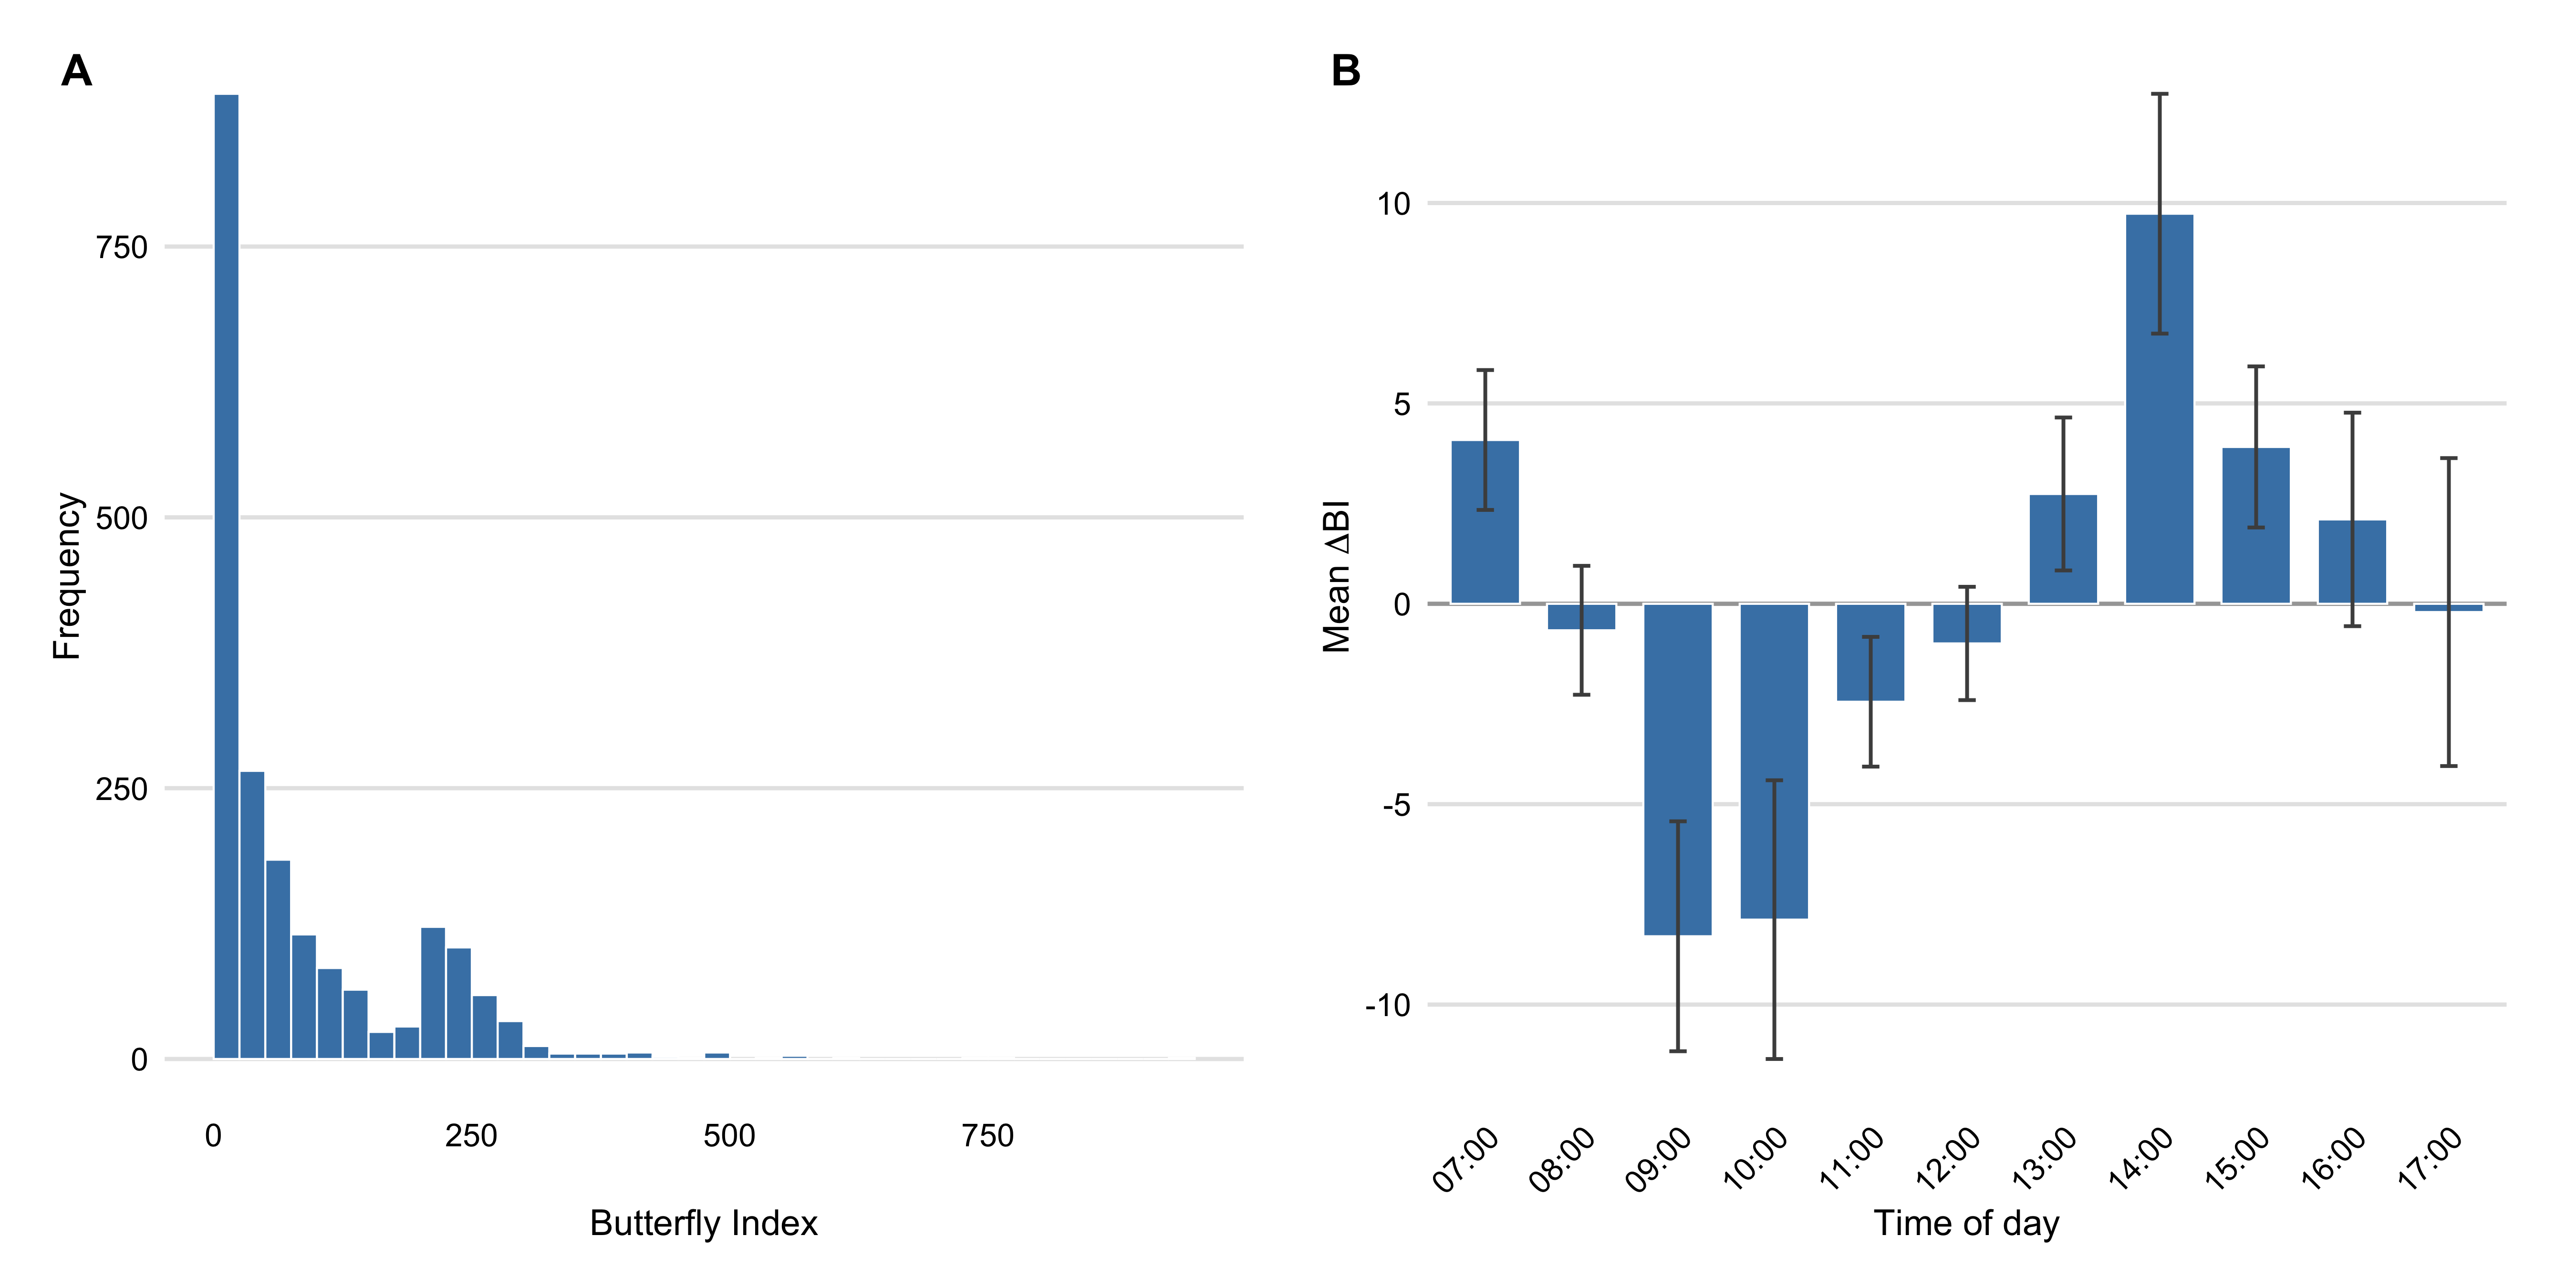
\includegraphics[width=0.95\textwidth]{figures/descriptive_bi.png}
\caption{Distribution of monarch abundance and 30-minute cluster change. BI is butterfly index. (A) Histogram of BI across 2,028 unique observation images. (B) Mean 30-minute $\Delta$BI by hour of the ending observation, based on available 1,894 paired intervals. Error bars show $\pm$1 SE across deployment-day hourly means.}
\label{fig:descriptive_bi}
\end{figure}

The Next Day Window analysis included 96 consecutive-day pairs with a mean interval of 29.8 hours. Previous-day maximum BI ranged from 0 to 770. Changes in daily maximum BI ranged from a loss of 376 to a gain of 464 (mean = $-$10.5 $\pm$ 112.2). Maximum gusts within these intervals ranged from 2.0 to 12.8~m/s (mean = 4.5 $\pm$ 1.8~m/s), and cumulative sun-exposed BI ranged from 0 to 1,122 (mean = 139.8 $\pm$ 206.9).

\subsection{30-Minute Wind Disruption Analysis}

To test whether wind was associated with short-term changes in visible cluster size, we compared 17 primary candidate models. The best-supported model included previous BI, time since sunrise, and a linear three-way interaction among maximum wind gust, average temperature, and sun-exposed BI. It received nearly all candidate-set support (AICc = 8052.02, Akaike weight $>$ 0.9999). The model containing all three linear two-way interactions ranked second and was 33.80 AICc units higher. The same environmental three-way interaction ranked first when previous BI was omitted and when time since sunrise was omitted.

The fitted relationship between maximum gust and short-term BI change varied with both temperature and sun-exposed BI. Evidence for this joint dependence was strong (three-way interaction, $\beta$ = 0.00651, SE = 0.00108, $t$ = 6.02, $p < 0.001$). The positive interaction term indicates that the conditional wind slope shifted toward more positive values as temperature increased, and that this shift was larger when sun-exposed BI was higher. When sun-exposed BI was zero, wind slopes were not distinguishable from zero at 10, 15, or 20$^{\circ}$C (all $p > 0.16$). At sun-exposed BI values of 7 and 20, slopes were negative at 10$^{\circ}$C (both $p < 0.001$) and positive at 20$^{\circ}$C (both $p < 0.001$). At 15$^{\circ}$C, the slope was not distinguishable from zero at sun-exposed BI of 7 ($p$ = 0.063) and was positive at sun-exposed BI of 20 ($p$ = 0.018), although predicted changes remained close to zero across the displayed gust range (Figure~\ref{fig:thirty_minute_response}).

Previous BI had a negative coefficient ($\beta$ = $-$0.00230, SE = 0.00048, $p < 0.001$), and time since sunrise had a small positive coefficient ($\beta$ = 0.00055, SE = 0.00027, $p$ = 0.041). These coefficients were treated as adjustments rather than biological effects. The selected model accounted for 5.3\% of the variation in short-term BI change. Residual diagnostics showed modest tail deviations from normality and little remaining temporal autocorrelation.

\begin{figure}[H]
\centering
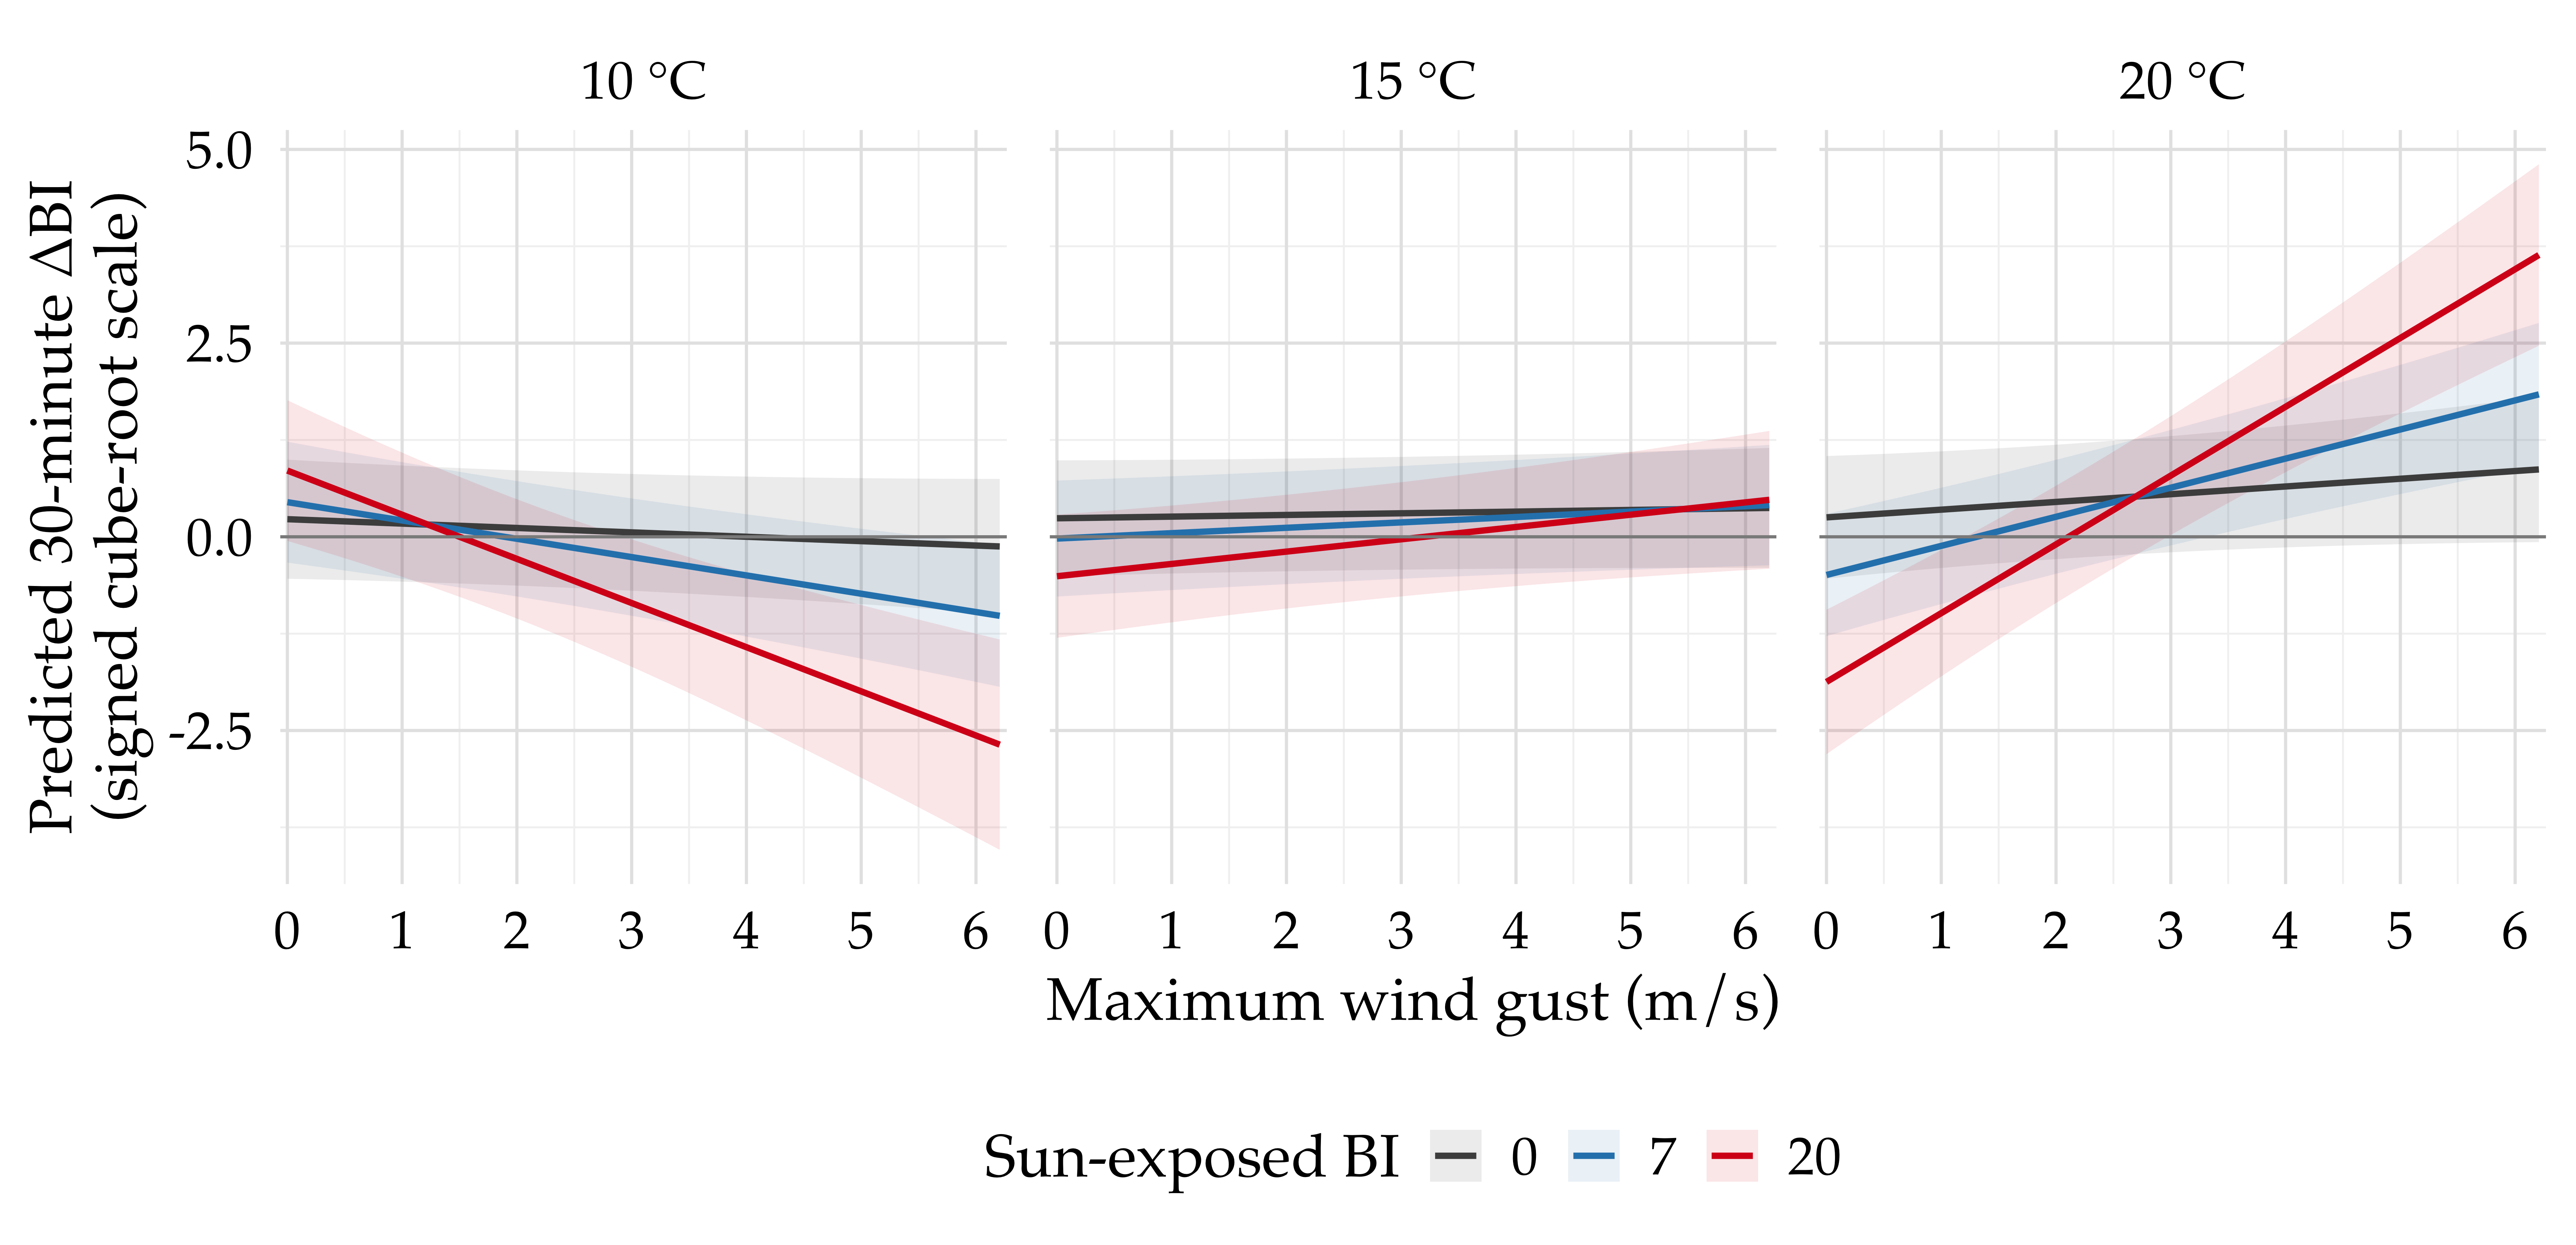
\includegraphics[width=0.98\textwidth]{analysis/outputs/harmonized_model_comparison/figures/thirty_minute_predicted_response.png}
\caption{Predicted 30-minute change in Butterfly Index (BI) across the three-way interaction among maximum wind gust, temperature, and sun-exposed BI. Predictions are shown on the signed cube-root $\Delta$BI scale, with pointwise 95\% confidence intervals shown by shading. Previous BI is held at its median of 37, and time since sunrise is held at its median of 300 minutes. Sun-exposed BI values of 7 and 20 represent the median and 75th percentile among observations with positive sun-exposed BI. Lines extend from 0 to the overall 99th percentile of observed maximum gust, 6.21~m/s. All observations were retained in model fitting.}
\label{fig:thirty_minute_response}
\end{figure}

\subsection{Next Day Window Analysis}

To test whether wind was associated with changes in visible cluster size over a longer response window, we compared 35 primary candidate models. The best-supported model included previous-day maximum BI, window duration, and a centered tensor interaction between maximum wind gust and cumulative sun-exposed BI (AICc = 650.01, Akaike weight = 0.368). A maximum-temperature-only model was also competitive ($\Delta$AICc = 1.89, Akaike weight = 0.143). A linear three-way interaction using temperature at the previous day's maximum BI ranked third ($\Delta$AICc = 2.99, Akaike weight = 0.082), and the adjustment-only model ranked fifth ($\Delta$AICc = 3.58, Akaike weight = 0.061). The centered tensor interaction remained first in the sensitivity analysis without previous BI, although a three-way interaction using maximum temperature was within one AICc unit ($\Delta$AICc = 0.81).

Within the selected model, predicted Next Day Window BI change varied across combinations of maximum wind gust and cumulative sun-exposed BI (edf = 6.68, $F$ = 4.10, $p < 0.001$). The interaction's fitted contribution was positive at low gust speeds and low cumulative sun-exposed BI, negative at similar gust speeds with higher cumulative sun-exposed BI, and positive across parts of the intermediate wind and sun-exposed BI range (Figure~\ref{fig:interaction_wind_sun_nextday}). Sparse regions outside the reliable interpolation area were not interpreted. Previous-day maximum BI had a negative coefficient ($\beta$ = $-$0.0297, SE = 0.0060, $p < 0.001$), whereas window duration was retained as an adjustment but was not supported ($\beta$ = $-$0.190, SE = 0.178, $p$ = 0.289). Because previous-day maximum BI contributed to the response definition, its coefficient was treated as an adjustment rather than interpreted as a biological effect.

The selected model accounted for 39.7\% of the variation in Next Day Window BI change. Residual and basis-dimension diagnostics did not indicate major model violations.

\begin{figure}[H]
\centering
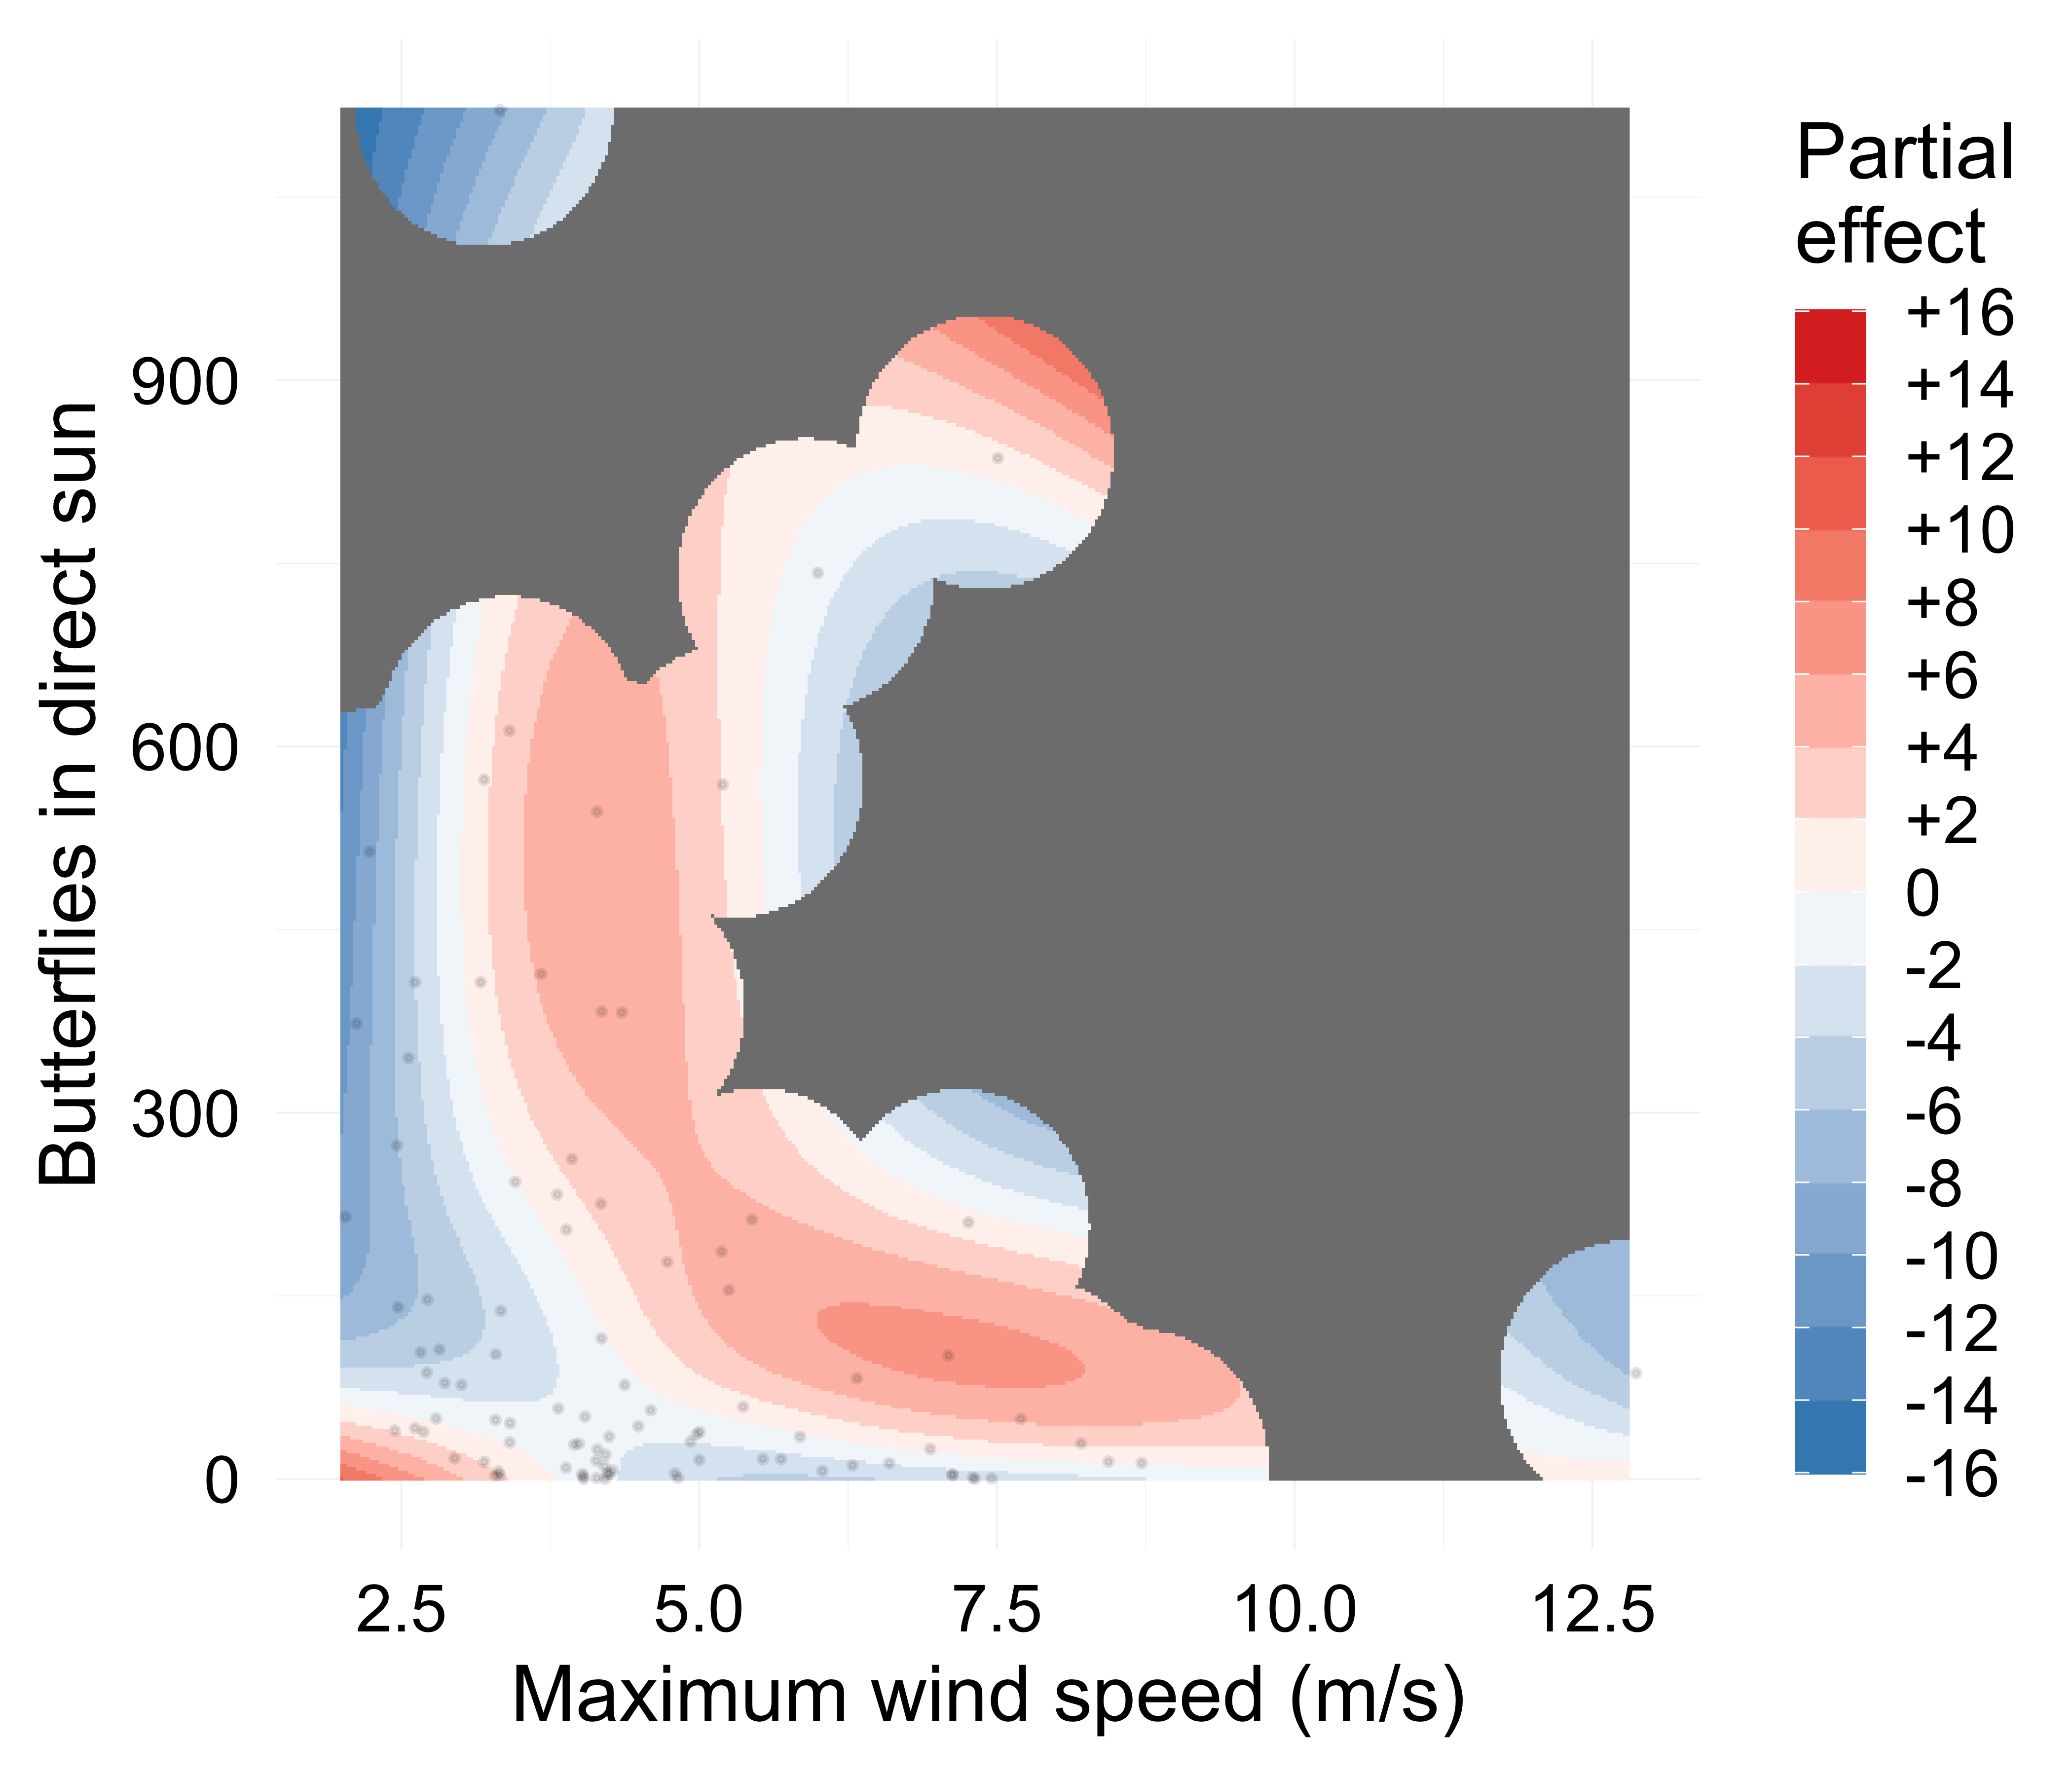
\includegraphics[width=0.72\textwidth]{analysis/outputs/next_day_window/figures/interaction_wind_sun_nextday.png}
\caption{Partial effect of the centered interaction between maximum wind gust and cumulative sun-exposed Butterfly Index (BI) on signed square-root transformed change in daily maximum BI. Positive and negative values indicate point estimates of the interaction's contribution to the fitted response, not full response predictions. The surface does not show local uncertainty. Jittered points show observed predictor combinations. Gray areas fall outside the supported interpolation region and were not interpreted.}
\label{fig:interaction_wind_sun_nextday}
\end{figure}

%% ------------------------------------------------------------------
\section{Discussion}
%% ------------------------------------------------------------------

For over three decades, the Wind Disruption Hypothesis has held that winds at or above approximately 2~m/s can physically dislodge overwintering monarchs or cause them to relocate, producing declines in cluster abundance as wind increases \cite{leongRestorationOverwinteringGrove1999,leongEvaluationManagementCalifornia2016}. We evaluated this prediction at two overwintering groves during one season by pairing nearby maximum wind gusts with subsequent changes in visible Butterfly Index over 30-minute and next-day response windows. Butterfly Index, hereafter BI, is an image-derived index of the number of butterflies visible within a fixed camera view rather than a complete count of the aggregation. We did not detect the consistently negative association expected under the commonly stated form of the Wind Disruption Hypothesis. Instead, the association between wind and visible cluster change depended on other biologically relevant conditions.

The 30-minute analysis provided the clearest evidence for this conditional relationship. The selected model included a three-way interaction among maximum wind gust, approximate local temperature, and sun-exposed BI. Sun-exposed BI was the portion of visible BI recorded in image cells receiving direct sunlight. When sun-exposed BI was zero, the association between maximum gust and BI change was not distinguishable from zero at representative temperatures of 10, 15, or 20$^{\circ}$C. Wind therefore had no detectable association with short-term cluster change when no butterflies were visible in direct sunlight. When sun-exposed BI was greater than zero, however, the association changed with temperature.

At 10$^{\circ}$C, increasing gusts were associated with declining BI, and this decline became steeper as sun-exposed BI increased. At 15$^{\circ}$C, predicted changes remained close to zero and their confidence intervals included zero throughout the displayed gust range. At 20$^{\circ}$C, increasing gusts were associated with increasing BI when sun-exposed BI was greater than zero. Under these warm and sunny conditions, fitted BI change was negative at low gust speeds and positive at higher gust speeds. Thus, the direction of the wind association changed across thermal and sun-exposure conditions rather than remaining consistently negative.

The Next Day Window analysis also identified a conditional association between maximum gust and sun-exposed BI. Its fitted response varied across combinations of maximum gust and cumulative sun-exposed BI rather than showing a uniformly negative wind relationship. This analysis contained 96 consecutive-day comparisons from one grove and had greater model-selection uncertainty than the 30-minute analysis. Three-way models were evaluated using each of the three Next Day temperature summaries. The three-way model using temperature at the previous day's maximum BI ranked third and was about three AICc units above the centered wind by sun-exposed BI interaction. The centered interaction also ranked first without adjustment for previous BI, although the maximum-temperature three-way model was then within one AICc unit. We therefore treat the selected Next Day relationship as complementary evidence that the relationship with wind was conditional, not as an independent replication of the specific three-way interaction found over 30 minutes.

Maximum gusts frequently exceeded the proposed 2~m/s threshold while butterflies remained visible. Among paired 30-minute observations with butterflies present, 57.9\% contained maximum gusts at or above 2~m/s. Every observation period in the Next Day Window analysis contained a recorded maximum gust at or above 2~m/s. These values were one-minute maximum gust records measured near the monitored clusters. They were not measurements of sustained exposure above 2~m/s at the butterflies themselves and therefore do not provide an exact test of the historical threshold formulation. Nevertheless, neither response window produced the consistent decline in visible cluster size expected under a simple wind-threshold model.

Previous work provides context for this departure from a single-threshold response. The Microclimate Hypothesis has commonly been interpreted as proposing that western monarch aggregations occupy a relatively uniform set of environmental conditions. Saniee and Villablanca \cite{sanieeHierarchyScaleInfluence2022} found instead that microclimatic attributes at aggregation locations varied geographically and that apparently suitable aggregation conditions occurred across substantial portions of individual groves. They concluded that overwintering habitat selection at local and geographic scales may be commingled when microclimate is treated as a single local envelope. Their study did not test wind or the physiological mechanisms underlying microclimate use. It nevertheless provides a broader context in which monarch responses may depend on interacting local conditions rather than universal environmental thresholds.

Previous physiological work offers one possible explanation for the conditional relationships observed here. Overwintering monarchs must conserve lipid reserves while maintaining the capacity for essential movement. Thoracic temperatures of approximately 12.7 to 16$^{\circ}$C are associated with powered flight, but direct solar exposure can warm monarchs above flight temperature even when ambient conditions are cooler \cite{mastersMonarchButterflyDanaus1988}. Solar basking may also provide an energetic advantage over shivering, which requires substantially more energy than resting \cite{kammerThoracicTemperatureShivering1970}. Under warmer conditions, however, direct sun can elevate body temperature enough to promote heat-avoidance behavior and additional movement. Wind may interact with both processes through convective heat transfer.

The 30-minute pattern is compatible with this thermoregulatory interpretation. At 10$^{\circ}$C, the negative wind association appeared only when butterflies were visible in sunlight. Solar warming may have allowed butterflies to move under otherwise restrictive ambient conditions, while wind altered the thermal value of exposed positions. At 15$^{\circ}$C, near the commonly reported flight-threshold range, little biologically interpretable change was associated with wind. At 20$^{\circ}$C, the transition from declining BI under low wind to increasing BI under higher wind is compatible with a balance between solar or ambient heat gain and convective cooling. Wind could provide passive cooling under warm, sunny conditions, allowing butterflies to remain at or move into exposed locations.

These interpretations remain hypotheses. The observed declines could represent thermally motivated movement, mechanical disturbance, movement to an unmonitored location, wind-driven changes in visibility, or another process. Likewise, increasing BI under warm and windy conditions does not demonstrate that butterflies actively sought wind or that convective cooling caused their arrival. We did not measure solar irradiance, thoracic temperature, convective heat transfer, metabolic expenditure, lipid depletion, or movement among roost locations.

We provisionally refer to the alternative explanation as the Physiological and Energetic Constraint Hypothesis. Under this hypothesis, monarch responses to wind depend on the net thermal and energetic consequences of wind, ambient temperature, and solar exposure rather than on wind speed alone. The same wind speed could therefore be unfavorable, neutral, or favorable under different thermal conditions. Direct evaluation requires simultaneous measurements of wind exposure at the butterflies, solar irradiance, ambient and body temperature, and movement among roost locations.

Several features of the study constrain the scope of inference. The data came from two blue gum eucalyptus groves on one installation during a single overwintering season. Nearly all 30-minute observations came from one grove, and only that grove contributed to the Next Day Window analysis. Deployments represented monitoring periods rather than independent biological populations, and some may have included the same aggregation or individual butterflies. The relatively small clusters observed during the study may also respond differently from the large, multilayered aggregations in which many butterflies attach primarily to other butterflies rather than directly to vegetation \cite{leongMicroenvironmentalFactorsAssociated1990,browerMonarchButterflyClusters2008}.

The measurements introduce additional uncertainty. Wind was measured near the clusters but was not validated at individual butterfly positions within the canopy. Camera temperatures were not independently calibrated against reference sensors. Sun-exposed BI depended on visible cluster size, butterfly behavior, visibility, and canopy geometry and was not a physical measurement of solar irradiance. Wind-driven branch movement could also redistribute a visible aggregation among image cells and introduce short-term error into BI change. Consequently, changes in visible BI cannot be interpreted as confirmed arrivals, departures, or physical dislodgment.

Within these constraints, the study does not support a simple formulation in which increasing wind consistently reduces overwintering cluster abundance. The principal finding is not that wind was unimportant, but that its association with visible cluster change depended on other biologically relevant conditions. An energetic interpretation provides a plausible and testable explanation for that conditionality, but establishing the mechanism will require direct physiological and microclimatic measurements.


%% ------------------------------------------------------------------
\section{Conclusions}
%% ------------------------------------------------------------------

Across the wind conditions measured at two overwintering groves during one season, we did not detect a consistent negative association between maximum wind gust and subsequent visible cluster change. The 30-minute association depended jointly on wind, approximate local temperature, and sun-exposed BI. The Next Day Window also supported a conditional wind by sun-exposed BI relationship, with greater model-selection uncertainty. Because one-minute maximum gust records do not measure sustained exposure above 2~m/s, this study does not provide an exact test of the historical threshold formulation.

The conditional patterns are compatible with a thermoregulatory explanation, but we did not measure thoracic temperature, solar irradiance, convective heat transfer, metabolic expenditure, or lipid depletion. Thermoregulation should therefore be treated as a hypothesis for future testing rather than as a demonstrated mechanism.

These findings arrive at a critical moment for monarch conservation. With western populations at historic lows, assumptions about habitat requirements deserve continued scrutiny. Our results do not justify removing existing wind-protection measures, but they do support testing whether management criteria based on a single wind-speed threshold adequately represent the environmental conditions used by overwintering monarchs. Conservation efforts should continue to preserve existing groves while direct physiological and multi-site studies evaluate alternative management criteria.


%% ------------------------------------------------------------------
%% Back matter
%% ------------------------------------------------------------------

\vspace{6pt}

\authorcontributions{Conceptualization, K.N., P.C.I., J.D.\ and F.X.V.; methodology, K.N., P.C.I., J.D.\ and F.X.V.; software, K.N.; validation, K.N.; formal analysis, K.N.; investigation, K.N.; resources, P.C.I.\ and F.X.V.; data curation, K.N.; writing---original draft preparation, K.N.\ and F.X.V.; writing---review and editing, K.N., P.C.I., J.D.\ and F.X.V.; visualization, K.N.; supervision, F.X.V.; project administration, K.N.\ and F.X.V.; funding acquisition, P.C.I., J.D.\ and F.X.V. All authors have read and agreed to the published version of the manuscript.}

\funding{This research was primarily funded by the U.S. Geological Survey (USGS) Geosciences and Environmental Change Science Center (Contract No. 140G0224P0194). Additional funding support was provided by The Xerces Society for Invertebrate Conservation, US Forest Service International Programs, Department of Defense Legacy Resource Management Program, and the College of Science and Mathematics at California State University, San Luis Obispo.}

\dataavailability{The data presented in this study are available on request from the corresponding author.}

\conflictsofinterest{The authors declare no conflict of interest. The funders had no role in the design of the study; in the collection, analyses, or interpretation of data; in the writing of the manuscript; or in the decision to publish the results.}

\acknowledgments{The authors wish to thank Emma Pelton of The Xerces Society for her role in organizing collaborative efforts and advancing study ideas. We also thank Jessica Griffiths of Vandenberg Space Force Base for facilitating site access and selection, Ashley Fisher of The Xerces Society for insights into monarch ecology, and Jenn Yost of California Polytechnic State University for her help with the review process. We thank undergraduate research assistants Skyler Meinholz, Vincent Rios, Emery Doornbos, and Kevin Untalan for photo labeling and field assistance. Finally, we thank Charis van der Heide of Althouse and Meade, Inc., Sara Cuadra-Vargas of The Xerces Society, and Stephanie Little of California State Parks for their contributions to the monthly collaborative working group on western monarch overwintering dynamics.}


%% ------------------------------------------------------------------
%% Appendices
%% ------------------------------------------------------------------

\appendixstart
\begin{appendix}

\section{Candidate Model Strategy}

Both analyses used a common set of environmental hypothesis templates. Let $C$ denote the required adjustment covariates, $W$ maximum gust, $S$ sun-exposed BI, and $T$ one temperature measure. Linear interactions followed marginality. Thus, a three-way interaction included all associated main effects and two-way interactions. Smooth candidates included both a centered tensor interaction and a hierarchical tensor interaction with marginal smooths.

\begin{table}[H]
\caption{Environmental predictors and adjustment covariates in the candidate comparisons.}
\label{tab:harmonized_predictors}
\begin{tabularx}{\textwidth}{@{}p{0.17\textwidth}XX@{}}
\toprule
\textbf{Role} & \textbf{30-minute window} & \textbf{Next Day Window} \\
\midrule
$C$ & Previous BI and minutes since sunrise & Previous-day maximum BI and window duration \\
$W$ & Maximum gust within the paired interval & Maximum gust within the response window \\
$S$ & Sun-exposed BI at the earlier image & Cumulative sun-exposed BI across daylight images \\
$T$ & Mean camera temperature between paired images & Minimum temperature, maximum temperature, or temperature at the previous day's maximum BI, evaluated in separate candidates \\
\bottomrule
\end{tabularx}
\end{table}

\begin{table}[H]
\caption{Shared hypothesis templates. Each temperature-dependent template was fitted once in the 30-minute analysis and separately for each of the three Next Day temperature summaries.}
\label{tab:harmonized_templates}
\begin{tabularx}{\textwidth}{@{}p{0.10\textwidth}p{0.34\textwidth}X@{}}
\toprule
\textbf{ID} & \textbf{Hypothesis} & \textbf{Fixed-effect structure} \\
\midrule
H00 & Controls only & $C$ \\
H01 & Wind & $C + W$ \\
H02 & Sun-exposed BI & $C + S$ \\
H03 & Additive wind and sun & $C + W + S$ \\
H04 & Linear wind by sun interaction & $C + W * S$ \\
H05 & Centered tensor interaction & $C + ti(W,S)$ \\
H06 & Additive wind and sun smooths & $C + s(W) + s(S)$ \\
H07 & Hierarchical tensor interaction & $C + s(W) + s(S) + ti(W,S)$ \\
T01 & Temperature & $C + T$ \\
T02 & Additive wind, temperature, and sun & $C + W + T + S$ \\
T03 & Wind by temperature & $C + W * T + S$ \\
T04 & Wind by sun, with temperature & $C + W * S + T$ \\
T05 & Temperature by sun, with wind & $C + T * S + W$ \\
T06 & All linear two-way interactions & $C + W * T + W * S + T * S$ \\
T07 & Full linear three-way interaction & $C + W * T * S$ \\
T08 & Additive environmental smooths & $C + s(W) + s(T) + s(S)$ \\
T09 & Smooth wind by sun interaction with temperature & $C + s(W) + s(T) + s(S) + ti(W,S)$ \\
\bottomrule
\end{tabularx}
\end{table}

\subsection{30-Minute Candidate Mapping}
\label{app:30min_models}

The primary 30-minute comparison contained the eight H templates and nine T templates, for 17 candidates. The adjustment set $C$ was previous BI and linear minutes since sunrise. The no-previous-BI sensitivity retained time since sunrise, and the no-time sensitivity retained previous BI. Each model included random intercepts for deployment and deployment-day and AR(1) correlation within deployment-day. All 51 fits completed without warnings. The full linear three-way interaction ranked first in all three candidate sets.

Table~\ref{tab:30min_candidates} gives the fixed-effect structure of every primary 30-minute candidate. In this table, $C_{30}$ is previous BI plus minutes since sunrise, $W_{30}$ is maximum gust within the paired interval, $S_{30}$ is sun-exposed BI at the earlier image, and $T_{30}$ is mean camera temperature between the paired images. Smooth terms used shrinkage thin-plate regression splines with $k=5$. Every candidate also had the random-effect and correlation structure described above.

\begin{longtable}{@{}p{0.13\textwidth}p{0.79\textwidth}@{}}
\caption{The 17 primary candidates in the 30-minute model comparison.} \label{tab:30min_candidates} \\
\toprule
\textbf{ID} & \textbf{Fixed-effect structure} \\
\midrule
\endfirsthead
\toprule
\textbf{ID} & \textbf{Fixed-effect structure} \\
\midrule
\endhead
H00 & $C_{30}$ \\
H01 & $C_{30} + W_{30}$ \\
H02 & $C_{30} + S_{30}$ \\
H03 & $C_{30} + W_{30} + S_{30}$ \\
H04 & $C_{30} + W_{30} * S_{30}$ \\
H05 & $C_{30} + ti(W_{30},S_{30})$ \\
H06 & $C_{30} + s(W_{30}) + s(S_{30})$ \\
H07 & $C_{30} + s(W_{30}) + s(S_{30}) + ti(W_{30},S_{30})$ \\
T01 & $C_{30} + T_{30}$ \\
T02 & $C_{30} + W_{30} + T_{30} + S_{30}$ \\
T03 & $C_{30} + W_{30} * T_{30} + S_{30}$ \\
T04 & $C_{30} + W_{30} * S_{30} + T_{30}$ \\
T05 & $C_{30} + T_{30} * S_{30} + W_{30}$ \\
T06 & $C_{30} + W_{30} * T_{30} + W_{30} * S_{30} + T_{30} * S_{30}$ \\
T07 & $C_{30} + W_{30} * T_{30} * S_{30}$ \\
T08 & $C_{30} + s(W_{30}) + s(T_{30}) + s(S_{30})$ \\
T09 & $C_{30} + s(W_{30}) + s(T_{30}) + s(S_{30}) + ti(W_{30},S_{30})$ \\
\bottomrule
\end{longtable}

\subsection{Next Day Candidate Mapping}
\label{app:nextday_models}

The primary Next Day comparison contained the eight H templates and nine T templates repeated for each of the three temperature summaries, for 35 candidates. The adjustment set $C$ was previous-day maximum BI and window duration. The no-previous-BI sensitivity removed previous-day maximum BI from all 35 candidates but retained window duration. Each model included a deployment random intercept and AR(1) correlation within deployment. All 70 fits completed without warnings. The centered wind by sun-exposed BI tensor interaction ranked first in both candidate sets.

Table~\ref{tab:nextday_candidates} gives the fixed-effect structure of every primary Next Day candidate. Here, $C_D$ is previous-day maximum BI plus window duration, $W_D$ is maximum gust within the response window, and $S_D$ is cumulative sun-exposed BI across daylight images. The three temperature variables are $T_{\min}$, minimum window temperature, $T_{\max}$, maximum window temperature, and $T_P$, temperature at the previous day's maximum BI. Smooth terms used shrinkage thin-plate regression splines with $k=5$. Every candidate also had the random-effect and correlation structure described above.

\begin{longtable}{@{}p{0.18\textwidth}p{0.74\textwidth}@{}}
\caption{The 35 primary candidates in the Next Day model comparison.} \label{tab:nextday_candidates} \\
\toprule
\textbf{ID} & \textbf{Fixed-effect structure} \\
\midrule
\endfirsthead
\toprule
\textbf{ID} & \textbf{Fixed-effect structure} \\
\midrule
\endhead
H00 & $C_D$ \\
H01 & $C_D + W_D$ \\
H02 & $C_D + S_D$ \\
H03 & $C_D + W_D + S_D$ \\
H04 & $C_D + W_D * S_D$ \\
H05 & $C_D + ti(W_D,S_D)$ \\
H06 & $C_D + s(W_D) + s(S_D)$ \\
H07 & $C_D + s(W_D) + s(S_D) + ti(W_D,S_D)$ \\
min-T01 & $C_D + T_{\min}$ \\
min-T02 & $C_D + W_D + T_{\min} + S_D$ \\
min-T03 & $C_D + W_D * T_{\min} + S_D$ \\
min-T04 & $C_D + W_D * S_D + T_{\min}$ \\
min-T05 & $C_D + T_{\min} * S_D + W_D$ \\
min-T06 & $C_D + W_D * T_{\min} + W_D * S_D + T_{\min} * S_D$ \\
min-T07 & $C_D + W_D * T_{\min} * S_D$ \\
min-T08 & $C_D + s(W_D) + s(T_{\min}) + s(S_D)$ \\
min-T09 & $C_D + s(W_D) + s(T_{\min}) + s(S_D) + ti(W_D,S_D)$ \\
max-T01 & $C_D + T_{\max}$ \\
max-T02 & $C_D + W_D + T_{\max} + S_D$ \\
max-T03 & $C_D + W_D * T_{\max} + S_D$ \\
max-T04 & $C_D + W_D * S_D + T_{\max}$ \\
max-T05 & $C_D + T_{\max} * S_D + W_D$ \\
max-T06 & $C_D + W_D * T_{\max} + W_D * S_D + T_{\max} * S_D$ \\
max-T07 & $C_D + W_D * T_{\max} * S_D$ \\
max-T08 & $C_D + s(W_D) + s(T_{\max}) + s(S_D)$ \\
max-T09 & $C_D + s(W_D) + s(T_{\max}) + s(S_D) + ti(W_D,S_D)$ \\
prev-T01 & $C_D + T_P$ \\
prev-T02 & $C_D + W_D + T_P + S_D$ \\
prev-T03 & $C_D + W_D * T_P + S_D$ \\
prev-T04 & $C_D + W_D * S_D + T_P$ \\
prev-T05 & $C_D + T_P * S_D + W_D$ \\
prev-T06 & $C_D + W_D * T_P + W_D * S_D + T_P * S_D$ \\
prev-T07 & $C_D + W_D * T_P * S_D$ \\
prev-T08 & $C_D + s(W_D) + s(T_P) + s(S_D)$ \\
prev-T09 & $C_D + s(W_D) + s(T_P) + s(S_D) + ti(W_D,S_D)$ \\
\bottomrule
\end{longtable}

All 121 fits were compared using maximum likelihood and AICc. Akaike weights were calculated separately within each response window and sensitivity framework. The selected formulas were refitted using restricted maximum likelihood. Complete machine-readable formulas, fit outcomes, rankings, and selected-model summaries accompany the analysis code.

\end{appendix}

%% ------------------------------------------------------------------
%% Bibliography
%% ------------------------------------------------------------------
\reftitle{References}
\bibliography{bibliography/references}

\end{document}
